\documentclass{article}

\textwidth=6.5in
\textheight=8.5in
\voffset=-54pt
\oddsidemargin=0in
\evensidemargin=0in
\setlength{\parskip}{8pt}
\setlength{\parindent}{0pt}

\usepackage{amsmath, amssymb}
\usepackage{ifthen}

\usepackage[inline]{enumitem}
\setlist{topsep=0pt, parsep=8pt}

\usepackage[rgb,table]{xcolor}\convertcolorsUfalse
\usepackage{graphicx}

% change hyperref options
\PassOptionsToPackage{hyphens}{url}
\usepackage[bookmarks,colorlinks,linkcolor=black,citecolor=blue,pdfstartview=FitH,urlcolor=blue]{hyperref}
\hypersetup{pdfpagemode=UseNone}
\usepackage{bookmark}

\usepackage{graphicx}
\usepackage{multicol}
\usepackage{framed}
\usepackage{array}

\usepackage{icomma}

\usepackage{soul}
\usepackage[normalem]{ulem}

\usepackage{pgfplots}
\pgfplotsset{compat=1.18}  
\pgfplotscreateplotcyclelist{mycolor}{black, blue, red, green!70!black, magenta, purple, cyan, orange }  
\pgfplotsset{
  disabledatascaling,
  cycle list=tikzcolor, 
  axis lines=middle,
  every axis plot/.style={no marks, thick},
  every axis/.style={
    enlarge x limits=false,
    enlarge y limits=auto,
    xlabel style={at={(current axis.right of origin)},anchor=west},
    ylabel style={at={(current axis.above origin)},anchor=south},
    % extra x and y ticks for asymptotes
    extra x tick style={grid=major, grid style={dashed,black}},
    extra y tick style={grid=major, grid style={dashed,black}},
    /pgf/number format/1000 sep={},
  },    
  tick label style = {font=\footnotesize, fill=\currentbgcolor, inner sep=0pt},    
  xticklabel shift=1pt,    
  scaled ticks=false,
  scaled y ticks=false,
  unbounded coords=jump,
  samples=101,
  minor tick length=0,
  scatter/classes={
    open={mark=*,draw=black,fill=white, mark size=2, thin},
    closed={mark=*,draw=black,fill=black, mark size=2, thin}
  },
  width=3in,
}
\pgfplotsset{open/.style={only marks, mark=*, fill=white, thin, mark size=2}}
\pgfplotsset{closed/.style={only marks, mark=*, draw=black, fill=black,
    thin, mark size=2}}
\pgfplotsset{labeled/.style={nodes near coords, only marks, mark=*, draw=black, fill=black, thin, mark size=2, point meta=explicit symbolic}}

\pgfplotsset{gridgraph/.style={clip=false, axis line style={shorten
      >=-8pt}, xlabel style={xshift=8pt}, ylabel style={yshift=8pt},
    enlargelimits=false, grid=major, tick style={black}}} 

\newcommand{\axes}[1][]{
  \begin{tikzpicture}
    \begin{axis}[xtick=\empty, ytick=\empty, ymin=-2, ymax=2,
      xmin=-4.25, xmax=4.25, #1]
    \end{axis}
  \end{tikzpicture}
}
\usepackage{tikz}
\usetikzlibrary{
  matrix,%
  % enables the snake paths
  decorations.pathmorphing,%
  % enables bigger arrows
  decorations.markings,%
  decorations.pathreplacing,%
  decorations.text,%
  calc,%
  patterns,%
  shapes.geometric,%
  arrows,
  decorations.shapes,
  positioning,
  plotmarks,
  intersections
}
\tikzset{>=latex} % sets default arrow type in tikz
\tikzset{font=\normalsize}
\tikzset{mark size=1.5pt, mark options=thin}
\tikzset{pin distance=4pt,
  every pin edge/.style={<-, thin, shorten <= -2pt}}

\interfootnotelinepenalty=10000
\renewcommand{\thefootnote}{(\arabic{footnote})}

\usepackage{multirow, bigdelim}

% change to \usepackage[sols]{handout} to see solutions
\usepackage[]{handout}

\newcommand\iscurrentenumi[1]{%
  \ifthenelse{\equal{#1}{\theenumi}}{}{#1}}
\setenumerate[1]{ref=\#\arabic*}
\setenumerate[2]{ref=\protect\iscurrentenumi{\theenumi}(\alph*)}
\newcommand\enumiiprefix[2]{%
  \ifthenelse{{\equal{#1}{\theenumi}}\AND{\equal{#2}{(\alph{enumii})}}}{}{}%
  \ifthenelse{{\equal{#1}{\theenumi}}\AND{\NOT{\equal{#2}{(\alph{enumii})}}}}{#2}{}%
  \ifthenelse{\equal{#1}{\theenumi}}{}{#1#2}%
}
\setenumerate[3]{ref=\protect\enumiiprefix{\theenumi}{(\alph{enumii})}\roman*}

\newlength{\tipmargin}
\makeatletter

\renewenvironment{framed}{
  \setlength{\tipmargin}{\textwidth-\linewidth}
  \advance\@totalleftmargin-\tipmargin
  \def\FrameCommand{\hspace{\tipmargin}\fbox}%
  \advance\linewidth\tipmargin
  \MakeFramed {\advance\hsize-\width \FrameRestore}%
}
{\endMakeFramed}

\makeatother

\definecolor{purple}{rgb}{0.5,0,1.0}

\definecolor{skyblue}{rgb}{0, 0.5, 1}

\usepackage{fancyhdr}
\lhead{\textcolor{white}{This content is protected and may not be shared, uploaded, or distributed.}}
\rhead{}
\rfoot{\vspace*{\fill}\footnotesize\textcopyright{} \emph{Harvard Math Ma}}
\renewcommand{\headrulewidth}{0pt}
\pagestyle{fancy}
\begin{document}

\htitle{Using Derivatives to Graph Functions}

\begin{problemonly}
  \begin{framed}

You should be able to:
    \begin{itemize}[topsep=0pt,partopsep=0pt,parsep=8pt,itemsep=0pt]

    \item Use the first derivative to determine where a function is
      increasing or decreasing and to find \emph{turning points}.

    \item Use the second derivative to determine where a function is
      concave up or concave down and to find \emph{inflection points}. 

    \item Put the above information together to sketch a reasonable graph
      of a function.

    \item Develop the habit of checking for consistency when putting several pieces of information together. 
    \end{itemize}
  \end{framed}
\end{problemonly}

\begin{enumerate}
\item 

  \note{I will start by having students try to reconstruct the table we made last time, since today is all about using those relationships.}

  \begin{problem}[\vfill\newpage]
    For a function $f(x)$, summarize the relationships among features (positive / negative, increasing / decreasing, etc.) of $f$, $f'$, and $f''$.
  \end{problem}  

  \begin{solution}
  \begin{center}
  \renewcommand{\arraystretch}{1.75}
  \begin{tabular}{| p{1.25in} | p{1.25in} | p{1.25in} |}
    \hline
    $f$ & $f'$ & \solonly{$\bm{f''}$} \\
    \hline\hline
    positive & & \\
    \hline
    negative & & \\
    \hline\hline
    increasing $\nearrow$ & \solonly{\textbf{positive}} & \\
    \hline
    decreasing $\searrow$ & \solonly{\textbf{negative}} & \\
    \hline\hline     
    concave up \tikz[scale=0.075] \draw (-2, 4) parabola bend (0, 0) (2, 4);  & \solonly{\textbf{increasing} $\bm{\nearrow}$} & \solonly{\textbf{positive}} \\
    \hline    
    concave down \tikz[scale=0.075] \draw (-2, -4) parabola bend (0, 0) (2, -4); & \solonly{\textbf{decreasing} $\bm{\searrow}$} & \solonly{\textbf{negative}} \\
    \hline
  \end{tabular}  
  \renewcommand{\arraystretch}{1}
  \end{center}
  \end{solution}

\item  \label{given-velocity-sketch-position-1}

  Albert is taking a very long car trip. Suppose that the following graph gives his velocity $v$ (measured in mph) as a function of time $t$ (measured in hours).

  \begin{tikzpicture}[
    declare function={
      f(\x) = (\x <= 4) * ( 36 - 9 * (\x - 2)^2)
      + and(4 < \x, \x <=6) * (456 - 216*\x + (63*\x^2)/2 - (3*\x^3)/2)
      + and(6 < \x, \x <= 10) * (-30); }]
    \begin{axis}[gridgraph, xtick={1, 2, ..., 10}, ytick={-40, -20, ...,
        40}, minor ytick={-50, -30, ..., 50}, ymin=-50, ymax=40,
      grid=both, width=\linewidth/2, xlabel=$t$, ylabel=$v$]
      \addplot+[domain=0:8] {f(x)};
    \end{axis}
  \end{tikzpicture}
  \axes[width=\linewidth/2, xlabel=$t$, ylabel=position, xmin=0, xmax=8.25,
  xtick={1, 2, ..., 8}]

  Let $A(t)$ be Albert's position at time $t$. 

  \begin{enumerate}

  \item \label{given-velocity-sketch-position-1-inc-dec}
    \begin{problem}[\vfill]
      Where is $A(t)$ increasing? Where is $A(t)$ decreasing?
    \end{problem}

    \begin{solution}
      To determine when Albert's position is increasing, we need to know
      when his velocity is positive. Looking at the velocity-time
      graph, we can produce the following sign chart for $A'(t)$. 

      \begin{center}
        \begin{tikzpicture}
          \draw[|-|] (0, 0) -- (8, 0);
          \node at (-0.5, 0) {$A'(t)$};
          \foreach \x in {0,4,8}
            \draw[shift={(\x,0)},color=black] (0pt,3pt) -- (0pt,-3pt) node[below] {$\x$};
          \node[circle, fill=black, inner sep=2pt] at (0,0) {};
          \node[circle, fill=black, inner sep=2pt] at (4,0) {};
          \node[above] at (2,0) {$+$};
          \node[above] at (6,0) {$-$};
        \end{tikzpicture}
      \end{center}

      Based on the sign chart for $A'(t)$, we can draw the following conclusions
      about $A(t)$. 

      \begin{itemize}
        \item $A(t)$ is increasing on $(0, 4)$ because $A'(t)$ is positive 
          on that interval.
        \item $A(t)$ is decreasing on $(4, 8)$ because $A'(t)$ is negative
          on that interval.
        \item $A(t)$ has horizontal tangents at
          $x=0$ and $x=4$, because $A'(t)$ is zero there.
      \end{itemize}

    \end{solution}

  \item \label{given-velocity-sketch-position-1-concavity}
    \begin{problem}[\vfill]
      Where is $A(t)$ concave up? Concave down? Are there places where it's neither?
    \end{problem}

    \begin{solution}
      To determine where the position-time graph would be concave up, we should
      figure out where Albert's acceleration is positive. To determine where
      Albert's acceleration is positive, we should look at where his velocity
      is increasing. Based on the velocity-time graph, we can produce the following
      sign chart for $A'(t)$.

      \begin{center}
        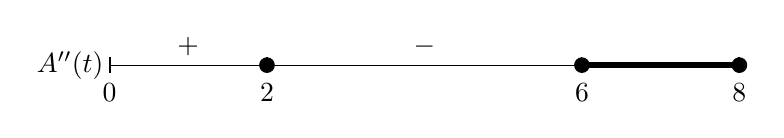
\begin{tikzpicture}
          \draw[|-|] (0, 0) -- (8, 0);
          \node at (-0.5, 0) {$A''(t)$};
          \foreach \x in {0,2,6,8}
            \draw[shift={(\x,0)},color=black] (0pt,3pt) -- (0pt,-3pt) node[below] {$\x$};
          \node[circle, fill=black, inner sep=2pt] at (2,0) {};
          \node[circle, fill=black, inner sep=2pt] at (6,0) {};
          \node[circle, fill=black, inner sep=2pt] at (8,0) {};
          \node[above] at (1,0) {$+$};
          \node[above] at (4,0) {$-$};
          \draw[line width=2pt, black] (6,0) -- (8,0);
        \end{tikzpicture}
      \end{center}

      Based on the sign chart for $A''(t)$, we can draw the following conclusions
      about $A(t)$.

      \begin{itemize}
        \item $A(t)$ is concave up on $(0,2)$ because $A''(t)$
          is positive on that interval.
        \item $A(t)$ is concave down on $(2,6)$ because $A''(t)$
          is negative on that interval.
        \item $A(t)$ is linear on $(6,8)$ because $A''(t)$ is zero
          on that interval.

      \end{itemize}
    \end{solution}

  \item \label{given-velocity-sketch-position-1-initial-condition-1}

    \note{I will encourage students to first summarize what they've found so far. For instance, $A(t)$ is increasing and concave up on $(0, 2)$, increasing and concave down on $(2, 4)$, and so on.}

    \begin{problem}[\vfill]
      Suppose that, at time 0, Albert is at position 0. On the axes above, sketch a graph of $A(t)$. The main thing to focus on is making your graph consistent with your answers to \ref{given-velocity-sketch-position-1-inc-dec} and \ref{given-velocity-sketch-position-1-concavity}. 
    \end{problem}

    \begin{solution}
      First, let's sketch a graph that's consistent with the information we found
      in part \ref{given-velocity-sketch-position-1-inc-dec}. We know that
      $A(t)$ should be increasing on $(0, 4)$ and decreasing on $(4, 8)$. 
      The tangent line at $x=4$ should be horizontal, but we'll smooth this out
      in the next step.
      
      \begin{center}
        \begin{tikzpicture}
          \begin{axis}[ytick=\empty, xlabel=$t$, ylabel=position, xmin=0, xmax=8.25, xtick={1, 2, ..., 8}]
            \addplot+[domain=0:4, dashed] {x};
            \addplot+[domain=4:8, dashed] {-1.1*x+8.4};
          \end{axis}
        \end{tikzpicture}
      \end{center}

      Note that the position graph we've drawn crosses the horizontal axis, but we don't
      know how to tell whether this should really happen and, if so, where. (We'll talk
      about this in Math Mb!)

      Now we can revise the graph to represent the information we found in part
      \ref{given-velocity-sketch-position-1-concavity}. We know that $A(t)$ should
      be concave up on $(0,2)$, concave down on $(2, 6)$ and linear on $(6, 8)$.
      
      \begin{center}
        \begin{tikzpicture}[declare function={f(\x)=and(6 < \x, \x <= 10)*(234 - 30*\x)+and(0 < \x, \x <= 4)*(-3*(-6 + \x)*\x^2)+and(4 < \x, \x <= 6)*(-0.375*(1536 - 1216*\x + 288*\x^2 - 28*\x^3 + \x^4));}]
          \begin{axis}[ytick=\empty, xlabel=$t$, ylabel=position, xmin=0, xmax=8.25, xtick={1, 2, ..., 8}, x=0.3in, y=0.015in]
            \addplot+[domain=0:8] {f(x)}; 
          \end{axis}
        \end{tikzpicture}
      \end{center}
      
    \end{solution}

  \item \label{given-velocity-sketch-position-1-initial-condition-2}

    \note{This is to help students realize that all antiderivatives of $v(t)$ are vertical shifts of each other. (I won't use the word antiderivative!)} 

    \begin{problem}[\vfill]
      Bart is also driving on the highway; at time 0, he's at position 10. By some miracle, his velocity graph is exactly the same as Albert's. Let $B(t)$ be Bart's position at time $t$, and sketch a graph of $B(t)$ on your graph from \ref{given-velocity-sketch-position-1-initial-condition-1}.
    \end{problem}

    \begin{solution}
      Since Albert and Bart are always driving with exactly the same velocity, $A(t)$
      and $B(t)$ will be increasing/decreasing and concave up/concave down on exactly
      the same intervals. However, the graphs will have different $y$-intercepts.
      So $B(t)$ will look like this: 
      \begin{center}
        \begin{tikzpicture}[declare function={f(\x)=and(6 < \x, \x <= 10)*(234 - 30*\x)+and(0 < \x, \x <= 4)*(-3*(-6 + \x)*\x^2)+and(4 < \x, \x <= 6)*(-0.375*(1536 - 1216*\x + 288*\x^2 - 28*\x^3 + \x^4));}]
          \begin{axis}[ytick=\empty, xlabel=$t$, ylabel=position, xmin=0, xmax=8.25, xtick={1, 2, ..., 8}, x=0.3in, y=0.015in]
            \addplot+[domain=0:8] {f(x)} node[pos=0.75, anchor=east]{$A(t)$}; 
            \addplot+[domain=0:8, skyblue] {f(x) + 10} node[pos=0.75, anchor=west]{$B(t)$}; 
          \end{axis}
        \end{tikzpicture}
      \end{center}
    \end{solution}

  \item
    \begin{problem}[\stretch{0.5}]
      How does $B(t)$ relate to $A(t)$? 
    \end{problem}

    \begin{solution}
      From the graphs, we can see that the graph of $B(t)$ is a vertical shift of 
      the graph of $A(t)$.
      If Bart always travels at the same velocity as Albert, then Bart will always
      be 10 miles ahead of Albert, so $B(t)=A(t)+10$.
    \end{solution}

  \end{enumerate}

\item 
  \begin{problem}[\nstretch{0.25}]
    Generalize: if $f'(t)$ is continuous and $f'(t) = g'(t)$, how does $g(t)$ relate to $f(t)$?
  \end{problem}

  \begin{solution}
    If $f$ and $g$ always have the same continuous derivative,
    then the graphs of $f(t)$ and $g(t)$ will be vertical shifts of each other. That is, $g(t) = f(t) + c$. Another
    way to say this is that $f(t)$ and $g(t)$ differ by a constant.
  \end{solution}

\item  

  \note{Now, we turn to an example where we have a formula for $f'$ rather than a graph.}

  In \href{https://people.math.harvard.edu/~jjchen/mathma/docs/homework/PS10.html}{Problem Set 10}, {{{{\#3}}(a)}}, you found that $\dfrac{d}{dx}(ax^2 + bx + c) = 2ax + b$. That will be useful in this problem!

  Suppose $f$ is an unknown function; all we know is that $f$ is continuous on $(-\infty, \infty)$ and $f'(x) = x^2 + x - 6$. ($x^2 + x - 6$ is also continuous on $(-\infty, \infty)$.)

  \begin{enumerate}
  \item

    \note{I will show them how to make a sign chart here.}

    \begin{problem}[\vfill]
      Where (for what values of $x$) is $f'(x)$ positive?
      Where is $f'(x)$ negative? What does this tell you about $f$?
    \end{problem}

    \begin{solution}
      If we had the graph of $y=f'(x)$, we could look at where the graph is above/below the $x$-axis
      to produce a sign chart, as we did in \#2. Since we don't have a graph, we can proceed by either
      1) sketching a rough graph or 2) creating a sign chart using algebra. 
      
      The first strategy
      works well for functions whose graphs are simple, 
      and the second strategy works better for functions whose graphs are more complex.
      We'll show both.

      Let's sketch a rough graph of $y=x^2+x-6$. Since this is a quadratic equation, we know that the graph
      will be a parabola. The graph will be concave up because the coefficient of $x^2$ is positive. We can
      factor to determine the $x$-intercepts: $y=(x+3)(x-2)$, so the $x$-intercepts are $-3$ and $2$.
      This means that the graph looks like this.

      \begin{center}
        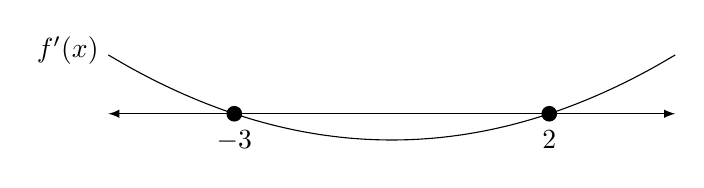
\begin{tikzpicture}[scale=0.8]
          \draw[<->] (-5,0) -- (4, 0);
          \draw[domain=-5:4, variable=\x, smooth] plot ({\x}, {(\x*\x + \x -6)/15});
          \node[left] at (-5,1) {$f'(x)$};
          \foreach \x in {-3,2}
            \draw[shift={(\x,0)},color=black] (0pt,3pt) -- (0pt,-3pt) node[below] {$\x$};
          \foreach \x in {-3,2}
            \node[circle, fill=black, inner sep=2pt] at (\x,0) {};
        \end{tikzpicture}
      \end{center}

      This gives us the following sign chart for $f'(x)$.

      \begin{center}
        \begin{tikzpicture}[scale=0.8]
          \draw[<->] (-5,0) -- (4, 0);
          \node[left] at (-5,0) {$f'(x)$};
          \foreach \x in {-3,2}
            \draw[shift={(\x,0)},color=black] (0pt,3pt) -- (0pt,-3pt) node[below] {$\x$};
          \foreach \x in {-3,2}
            \node[circle, fill=black, inner sep=2pt] at (\x,0) {};
          \node[above] at (-4,0) {$+$};
          \node[above] at (-0.5,0) {$-$};
          \node[above] at (3,0) {$+$};
        \end{tikzpicture}
      \end{center}
      

      To create a sign chart using algebra, we first need to determine the $x$-values for which $f'(x)$
      is zero or undefined. 
      As $f'(x)=x^2+x-6$, there are no $x$-values where $f'(x)$ is undefined. To find the $x$-values where
      $f'(x)$ is zero, we can set $f'(x)$ equal to zero and solve for $x$.
      \begin{align*}
        x^2 + x - 6 &= 0 \\
        (x+3)(x-2) &= 0
      \end{align*}
      From here, we can see that the $x$-values where $f'(x)$ is zero are $x=-3$ and $x=2$. We will mark
      these on our sign chart.
      \begin{center}
        \begin{tikzpicture}[scale=0.8]
          \draw[<->] (-5,0) -- (4, 0);
          \node[left] at (-5,0) {$f'(x)$};
          \foreach \x in {-3,2}
            \draw[shift={(\x,0)},color=black] (0pt,3pt) -- (0pt,-3pt) node[below] {$\x$};
          \foreach \x in {-3,2}
            \node[circle, fill=black, inner sep=2pt] at (\x,0) {};
        \end{tikzpicture}
      \end{center}
      We can see that our sign chart is now divided into 3 intervals: $(-\infty, -3)$, $(-3, 2)$, and $(2, \infty)$.
      We need to determine the sign of $f'(x)$ on each of these intervals. To do this, we can test 
      the value of $f'(x)$ at one $x$-value
      in each interval.
      \begin{alignat*}{3}
        f'(-4) &= (-4+3)(-4-2) &= (-1)(-6) &= +6 \\
        f'(0)  &= (0+3)(0-2)   &= (+3)(-2) &= -6 \\
        f'(3)  &= (3+3)(3-2)   &= (+6)(+1) &= +6
      \end{alignat*}
      Finally, we can represent this information on our sign chart.
      \begin{center}
        \begin{tikzpicture}[scale=0.8]
          \draw[<->] (-5,0) -- (4, 0);
          \node[left] at (-5,0) {$f'(x)$};
          \foreach \x in {-3,2}
            \draw[shift={(\x,0)},color=black] (0pt,3pt) -- (0pt,-3pt) node[below] {$\x$};
          \foreach \x in {-3,2}
            \node[circle, fill=black, inner sep=2pt] at (\x,0) {};
          \node[above] at (-4,0) {$+$};
          \node[above] at (-0.5,0) {$-$};
          \node[above] at (3,0) {$+$};
        \end{tikzpicture}
      \end{center}

      With both of these strategies, we find that $f'(x)$ is negative on the interval $(-3, 2)$ and positive
      on $(-\infty, -3) \cup (2, \infty)$. This tells us:
      \begin{itemize}
        \item $f$ is decreasing on $(-3, 2)$ because $f'$ is negative on that interval
        \item $f$ is increasing on $(-\infty, -3)$ and on $(2, \infty)$ because $f'$ is positive on those intervals
        \item $f$ has horizontal tangents at $x=-3$ and $x=2$ because $f'$ is zero there
      \end{itemize}
    \end{solution}

  \item
    \begin{problem}[\vfill]
      Find $f''$ and make a sign chart for $f''$. What does this tell you about $f$? 
    \end{problem}

    \begin{solution}
      We know that $f'(x) = x^2 + x - 6$. To find $f''(x)$, we need to take the derivative of $f'$. Using the
      formula $\dfrac{d}{dx}(ax^2 + bx + c) = 2ax + b$, we get $f''(x) = 2x+1$. To make a sign chart for $f''$,
      we can either sketch a rough graph or use algebra. Let's sketch a rough graph, since $f''$ is just a linear
      function.

      The graph of $y=2x+1$ is a straight line with a positive slope.
      To find the $x$-intercept, we can set $y=0$ and solve for $x$
      to get that the $x$-intercept is $-\frac{1}{2}$.
      \begin{center}
        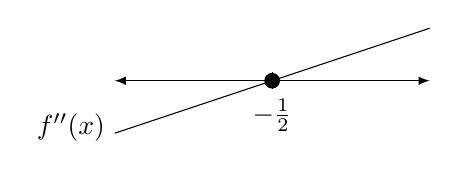
\begin{tikzpicture}[xscale=2]
          \draw[<->] (-1.5,0) -- (0.5,0);
          \draw[domain=-1.5:0.5, variable=\x, smooth] plot ({\x}, {(2*\x + 1)/3});
          \node[left] at (-1.5,-0.6) {$f''(x)$};
          \draw[shift={(-0.5,0)},color=black] (0pt,3pt) -- (0pt,-3pt) node[below] {$-\frac{1}{2}$};
          \node[circle, fill=black, inner sep=2pt] at (-0.5,0) {};
        \end{tikzpicture}
      \end{center}
      This gives us the following sign chart.
      \begin{center}
        \begin{tikzpicture}[xscale=2]
          \draw[<->] (-1.5,0) -- (0.5,0);
          \node[left] at (-1.5,0) {$f''(x)$};
          \draw[shift={(-0.5,0)},color=black] (0pt,3pt) -- (0pt,-3pt) node[below] {$-\frac{1}{2}$};
          \node[circle, fill=black, inner sep=2pt] at (-0.5,0) {};
          \node[above] at (-1,0) {$-$};
          \node[above] at (0,0) {$+$};
        \end{tikzpicture}
      \end{center}
      From the sign chart, we can see that $f''(x)$ is negative on $(-\infty, -\frac{1}{2})$ and positive
      on $(-\frac{1}{2}, \infty)$. This tell us:
      \begin{itemize}
        \item $f$ is concave down on $(-\infty, -\frac{1}{2})$ because $f''$ is negative on that interval
        \item $f$ is concave up on $(-\frac{1}{2}, \infty)$ because $f''$ is positive on that interval
      \end{itemize}
    \end{solution}
    

  \item
    \begin{problem}[\stretch{0.3}]
      Values of $x$ in the domain of $f$ where $f(x)$ switches from increasing to decreasing or vice versa are called \uline{turning points}. What are the turning points of $f$? 
    \end{problem}

    \begin{solution}
      Let's look again at the sign chart for $f'(x)$. 
      \begin{center}
        \begin{tikzpicture}[scale=0.8]
          \draw[<->] (-5,0) -- (4, 0);
          \node[left] at (-5,0) {$f'(x)$};
          \foreach \x in {-3,2}
            \draw[shift={(\x,0)},color=black] (0pt,3pt) -- (0pt,-3pt) node[below] {$\x$};
          \foreach \x in {-3,2}
            \node[circle, fill=black, inner sep=2pt] at (\x,0) {};
          \node[above] at (-4,0) {$+$};
          \node[above] at (-0.5,0) {$-$};
          \node[above] at (3,0) {$+$};
        \end{tikzpicture}
      \end{center}

      We can see that $f'(x)$ changes from positive to negative at $x=-3$, which means $f$ changes from increasing
      to decreasing at $x=-3$. And $f'(x)$ changes from negative to positive at $x=2$, so $f$ changes from decreasing
      to increasing at $x=2$. Both $x=-3$ and $x=2$ are in the domain of $f$. 
      Therefore $f$ has turning points at $x=-3$ and $x=2$. 
    \end{solution}

  \item

    \note{This is the last part on the worksheet that introduces new material.} 

    \begin{problem}[\nstretch{0.3}]
      Values of $x$ in the domain of $f$ where $f(x)$ switches from concave up to concave down or vice versa are called \uline{inflection points}. What are the inflection points of $f$? 
    \end{problem}

    \begin{solution}
      Let's look again at the sign chart for $f''(x)$. 

     \begin{center}
        \begin{tikzpicture}[xscale=2]
          \draw[<->] (-1.5,0) -- (0.5,0);
          \node[left] at (-1.5,0) {$f''(x)$};
          \draw[shift={(-0.5,0)},color=black] (0pt,3pt) -- (0pt,-3pt) node[below] {$-\frac{1}{2}$};
          \node[circle, fill=black, inner sep=2pt] at (-0.5,0) {};
          \node[above] at (-1,0) {$-$};
          \node[above] at (0,0) {$+$};
        \end{tikzpicture}
      \end{center}

        We can see that $f''(x)$ changes from negative to positive at $x=-\frac{1}{2}$, which means $f$ changes
        from concave down to concave up at $x=-\frac{1}{2}$. Also, $x=-\frac{1}{2}$ is in the domain of $f$.
        Therefore $f$ has an inflection point at $x=-\frac{1}{2}$. 
    \end{solution}

  \item
    \begin{problem}[\vfill]
      Sketch a possible graph of $f$ (that's consistent with your answers so far).
    \end{problem}

    \begin{solution}
      First, let's sketch a graph that's consistent with the information we found in part (a). We know
      $f$ should be increasing on $(-\infty, -3)$, decreasing on $(-3, 2)$, and increasing on $(2, \infty)$.
      There should be horizontal tangents at the turning points, but we'll smooth those out later.

      \begin{center}
        \begin{tikzpicture}
          \begin{axis}[ytick=\empty, xtick={-3, 2}]
            \addplot+[domain=-5:-3, dashed] {x+6};
            \addplot+[domain=-3:2, dashed] {-x};
            \addplot+[domain=2:4, dashed] {x-4};
          \end{axis}
        \end{tikzpicture}
      \end{center}

     Note that we don't know where the $x$-intercept(s) or $y$-intercept actually are.

     Now let's revise our graph to represent the information we found in part (b). We know that $f$ should
     be concave down on $(-\infty, -\frac{1}{2})$ and concave up on $(-\frac{1}{2}, \infty)$. 
     \begin{center}
        \begin{tikzpicture}
          \begin{axis}[ytick=\empty, xtick={-3, -0.5, 2}, xticklabels={$-3$, $-\frac{1}{2}$, $2$}]
            \addplot+[domain=-5:4] {x^3/3 + x^2/2 -6*x};
          \end{axis}
        \end{tikzpicture}
      \end{center}
      
    \end{solution}

  \item

    \note{This is just to emphasize again that knowing $f'$ only tells us about $f$ up to a vertical shift.}

    \begin{problem}[\vfill]
      How many zeros ($x$-intercepts) could $f$ possibly have? Sketch a possible graph for each possible number of zeros. How do the different possibilities relate to each other?
    \end{problem}

    \begin{solution}
      The graph of $f$ could differ from the one we sketched in part (e) by some vertical shift. That means
      we have these possibilities:
      \begin{itemize}
        \item 3 $x$-intercepts
        
        \begin{tikzpicture}
          \begin{axis}[ytick=\empty, xtick={-3, -0.5, 2}, xticklabels={$-3$, $-\frac{1}{2}$, $2$}, width=2in]
            \addplot+[domain=-6:4] {x^3/3 + x^2/2 -6*x};
            \addplot[closed] coordinates {(-5.058, 0) (0, 0) (3.558, 0)};
          \end{axis}
        \end{tikzpicture}

      \item 2 $x$-intercepts

        \begin{tikzpicture}
          \begin{axis}[ytick=\empty, xtick={-3, -0.5, 2}, xticklabels={$-3$, $-\frac{1}{2}$, $2$}, width=2in]
            \addplot+[domain=-6:4] {x^3/3 + x^2/2 -6*x + 22/3};
            \addplot[closed] coordinates {(-5.5, 0) (2,0)};
          \end{axis}
        \end{tikzpicture}

      \item 1 $x$-intercept

        \begin{tikzpicture}
          \begin{axis}[ytick=\empty, xtick={-3, -0.5, 2}, xticklabels={$-3$, $-\frac{1}{2}$, $2$}, width=2in]
            \addplot+[domain=-6:4] {x^3/3 + x^2/2 -6*x + 10};
            \addplot[closed] coordinates {(-5.637, 0)};
          \end{axis}
        \end{tikzpicture}

      \end{itemize}
      Therefore $f$ could have 1, 2, or 3 $x$-intercepts.
    \end{solution}
  \end{enumerate}

\item  

  Suppose $f$ is an unknown function with domain $(0, \infty)$; we know $f(x)$ has a vertical asymptote at $x = 0$ and that $f'(x) = x - \dfrac{4}{x}$.
  \begin{enumerate}
  \item
    \begin{problem}[\vfill\newpage]
      Where is $f$ increasing? Where is $f$ decreasing? What are the turning points of $f$?
    \end{problem}

    \begin{solution}
      To determine where $f$ is increasing/decreasing, we need to determine where $f'$ is positive/negative, so
      we should go through the process of making a sign chart for $f'(x)=x-\frac{4}{x}$. This function
      doesn't have a simple graph, so we should make the sign chart using algebra.

      First, we need to determine where $f'(x)$ is zero or undefined. We can see that $f'(x)$ is undefined
      when $x=0$. To find for the $x$-values for which $f'(x)$, we set $f'(x)=0$ and solve for $x$. 
      \begin{align*}
        x - \frac{4}{x} &= 0 \\
        \frac{x^2-4}{x} &= 0 \\
        \frac{(x+2)(x-2)}{x} &= 0 
      \end{align*}
      From here, we can see that $f'(x)$ will be zero at $x=-2$ and $x=2$. Since the domain of $f$ is
      $(0, \infty)$, we'll discard $x=-2$ and just represent $x=0$ and $x=2$ on our sign chart.

      \begin{center}
        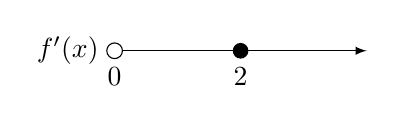
\begin{tikzpicture}[scale=0.8]
          \draw[->] (0,0) -- (4, 0);
          \node[left] at (-0.1,0) {$f'(x)$};
          \foreach \x in {0,2}
            \draw[shift={(\x,0)},color=black] (0pt,3pt) -- (0pt,-3pt) node[below] {$\x$};
          \node[circle, fill=black, inner sep=2pt] at (2,0) {};
          \node[circle, draw=black, fill=white, inner sep=2pt] at (0,0) {};
        \end{tikzpicture}
      \end{center}

      
      Now we need to determine the sign of $f'(x)$ on each interval. We'll do this by testing 
      the value of $f'(x)$ at one $x$-value
      in each interval.
      \begin{alignat*}{3}
        f'(1) &= 1-4 &= -3 \\
        f'(4) &= 4-1 &= +3
      \end{alignat*}

      Now we can complete our sign chart. 

      \begin{center}
        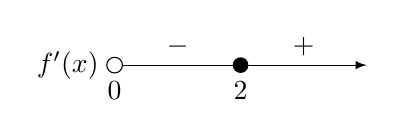
\begin{tikzpicture}[scale=0.8]
          \draw[->] (0,0) -- (4, 0);
          \node[left] at (-0.1,0) {$f'(x)$};
          \foreach \x in {0,2}
            \draw[shift={(\x,0)},color=black] (0pt,3pt) -- (0pt,-3pt) node[below] {$\x$};
          \node[circle, fill=black, inner sep=2pt] at (2,0) {};
          \node[circle, draw=black, fill=white, inner sep=2pt] at (0,0) {};
          \node[above] at (1,0) {$-$};
          \node[above] at (3,0) {$+$};
        \end{tikzpicture}
      \end{center}

      From this sign chart, we can determine that
      \begin{itemize}
        \item $f$ is decreasing on $(0, 2)$ since $f'$ is negative on that interval
        \item $f$ is increasing on $(2, \infty)$ since $f'$ is positive on that interval
        \item $f$ has a horizontal tangent at $x=2$ since $f'$ is zero there
        \item $f$ has a turning point at $x=2$ since $f$ changes from decreasing to increasing there and $x=2$
          is in the domain of $f$
      \end{itemize}
    \end{solution}

  \item

    \note{If we get to this problem, I probably won't actually have students spend the time to calculate $f''$. Instead, once they've written the limit definition correctly, I'll tell them the result.}

    \begin{problem}[\stretch{2.5}]
      Use the definition of the derivative to calculate $f''(x)$. 
    \end{problem}

    \begin{solution}
      Since $f''$ is the derivative of $f'$, let's write down the definition of the derivative.
      \begin{align*}
        f''(x) &= \lim_{h \to 0} \frac{f'(x+h)-f'(x)}{h} \\
        &= \lim_{h \to 0} \frac{x+h -\frac{4}{x+h} - \bigl(x - \frac{4}{x}\bigr)}{h} \\
        &= \lim_{h \to 0} \frac{h - \frac{4}{x+h} + \frac{4}{x}}{h} \\
        \intertext{Now let's rewrite the complex fraction a bit.}
        &= \lim_{h \to 0} \left(h-\frac{4}{x+h} + \frac{4}{x}\right)\cdot \frac{1}{h} \\
        &= \lim_{h \to 0} \left(h-\frac{4x}{x(x+h)} + \frac{4(x+h)}{x(x+h)}\right)\cdot \frac{1}{h} \\
        &= \lim_{h \to 0} \left(h+\frac{-4x+4(x+h)}{x(x+h)}\right)\cdot \frac{1}{h} \\
        &= \lim_{h \to 0} \left(h+\frac{4h}{x(x+h)}\right)\cdot \frac{1}{h} \\
        \intertext{Now we can cancel the $h$'s and evaluate the limit.}
        &= \lim_{h \to 0} \left( 1 + \frac{4}{x(x+h)}\right) \\
        &= 1 - \frac{-4}{x(x+0)} \\
        &= \boxed{1 + \frac{4}{x^2}}
      \end{align*}
    \end{solution}

  \item

    \note{There are no points where $f'' = 0$, so students will probably be confused about how to make a sign chart.}

    \begin{problem}[\vfill]
      Where is $f$ concave up? Where is concave down? What are the inflection points of $f$? 
    \end{problem}

    \begin{solution}
      Let's use algebra to make a sign chart for $f''(x)=1+\frac{4}{x^2}$. First, we need to determine
      where $f''(x)$ is zero or undefined. We can see that $f''(x)$ is undefined when $x=0$. We can solve
      for when $f''(x)=0$. 
      \begin{align*}
        1+\frac{4}{x^2} &= 0 \\
        \frac{x^2 + 4}{x^2} &= 0
      \end{align*}
      From here, we can see that the numerator is always positive and never equals zero, so there are no $x$-values
      for which $f''(x)$ is zero. This means our sign chart looks like this.
      
      \begin{center}
        \begin{tikzpicture}[scale=0.8]
          \draw[->] (0,0) -- (4, 0);
          \node[left] at (-0.1,0) {$f''(x)$};
          \foreach \x in {0}
            \draw[shift={(\x,0)},color=black] (0pt,3pt) -- (0pt,-3pt) node[below] {$\x$};
          \node[circle, draw=black, fill=white, inner sep=2pt] at (0,0) {};
        \end{tikzpicture}
      \end{center}
      
      Now we need to determine the sign of $f''(x)$ on the one interval. We can do this by testing
      the value of $f''(x)$ at an $x$-value in the interval.
      \[f''(1) = 1 + 4 = +5\]
      So our completed sign chart looks like this.

      \begin{center}
        \begin{tikzpicture}[scale=0.8]
          \draw[->] (0,0) -- (4, 0);
          \node[left] at (-0.1,0) {$f''(x)$};
          \foreach \x in {0}
            \draw[shift={(\x,0)},color=black] (0pt,3pt) -- (0pt,-3pt) node[below] {$\x$};
          \node[circle, draw=black, fill=white, inner sep=2pt] at (0,0) {};
          \node[above] at (2,0) {$+$};
        \end{tikzpicture}
      \end{center}
      Looking at our sign chart, we can conclude that:
      \begin{itemize}
        \item $f$ is concave up on $(0, \infty)$ because $f''$ is positive on that interval
        \item $f$ is not concave down on any interval because $f''$ is never negative
        \item $f$ has no inflection points because $f$ doesn not change concavity
      \end{itemize}

    \end{solution}

  \item
    \begin{problem}[\vfill\newpage]
      Sketch a possible graph of $f$. 
    \end{problem}

    \begin{solution}
      First, let's sketch a graph that's consistent with the information we found in part (a). We know
      $f$ should be decreasing on $(0, 2)$ and increasing on $(2, \infty)$. We also know that
      there is a vertical asymptote at $x=0$. 
      There should be a horizontal tangent at the turning point, but we'll smooth it out later.

      \begin{center}
        \begin{tikzpicture}
          \begin{axis}[ytick=\empty, xtick={0,2}, extra x ticks={0}, restrict y to domain=-5:5, width=2.5in]
            \addplot+[domain=0:2, dashed] {1/x};
            \addplot+[domain=2:4, dashed] {x-1.5};
          \end{axis}
        \end{tikzpicture}
      \end{center}

     Note that we don't know where the $x$-intercept(s) or $y$-intercept actually are.

     Now let's revise our graph to represent the information we found in part (c). We know that $f$ should
     be concave up on $(0, \infty)$. 
     \begin{center}
        \begin{tikzpicture}
          \begin{axis}[ytick=\empty, xtick={2}, width=2.5in]
            \addplot+[domain=0:4] {x^2/2 - 4*ln(x) + 2};
          \end{axis}
        \end{tikzpicture}
      \end{center}
      
    \end{solution}

  \end{enumerate}

\item  

  Suppose $f$ is an unknown function that's continuous on $(-\infty, \infty)$ and $f'(x) = x^3 - 8$.

  \begin{enumerate}
  \item

    \begin{problem}[\vfill]
      Where is $f$ increasing? Where is $f$ decreasing? What are the turning points of $f$? 
    \end{problem}

    \begin{solution}
      Let's make a sign chart for $f'(x)=x^3-8$. We can do this by sketching a rough graph. The graph
      of $y=x^3-8$ is the graph of $y=x^3$ but shifted down by 8 units. The $x$-intercept will be at $x=2$.

      \begin{center}
        \begin{tikzpicture}[yscale=0.05]
          \draw[<->] (-2,0) -- (4, 0);
          \draw[domain=-2:3.5, variable=\x, smooth] plot ({\x}, {(\x*\x*\x -8)});
          \node[left] at (-2,-15) {$f'(x)$};
          \foreach \x in {2}
            \draw[shift={(\x,0)},color=black] (0pt,3pt) -- (0pt,-3pt) node[below] {$\x$};
          \foreach \x in {2}
            \node[circle, fill=black, inner sep=2pt] at (\x,0) {};
        \end{tikzpicture}
      \end{center}

      This gives us the following sign chart.

      \begin{center}
        \begin{tikzpicture}[yscale=0.05]
          \draw[<->] (-2,0) -- (4, 0);
          \node[left] at (-2,0) {$f'(x)$};
          \foreach \x in {2}
            \draw[shift={(\x,0)},color=black] (0pt,3pt) -- (0pt,-3pt) node[below] {$\x$};
          \foreach \x in {2}
            \node[circle, fill=black, inner sep=2pt] at (\x,0) {};
          \node[above] at (0,0) {$-$};
          \node[above] at (3,0) {$+$};
        \end{tikzpicture}
      \end{center}

      From the sign chart, we can conclude that:
      \begin{itemize}
        \item $f$ is decreasing on $(-\infty, 2)$, since $f'$ is negative on that interval
        \item $f$ is positive on $(2, \infty)$, since $f'$ is positive on that interval
        \item $f$ has a horizontal tangent at $x=2$, since $f'$ is zero there
        \item $f$ has a turning point at $x=2$, since $f$ changes from decreasing to increasing there and $x=2$
          is in the domain of $f$
      \end{itemize}
    \end{solution}
  \end{enumerate}

  It turns out that $f''(x) = 3x^2$. (For extra practice, use the definition of the derivative to show this!)

  \begin{enumerate}[resume]

  \item

    \note{Although there is a point where $f''(x) = 0$, it isn't an inflection point.}

    \begin{problem}[\vfill]
      Where is $f$ concave up? Where is concave down? What are the inflection points of $f$? 
    \end{problem}

    \begin{solution}
      Let's make a sign chart for $f''(x)=3x^2$. We can do this by sketching a rough graph.
      \begin{center}
        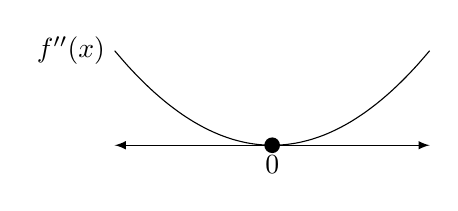
\begin{tikzpicture}[yscale=0.1]
          \draw[<->] (-2,0) -- (2, 0);
          \draw[domain=-2:2, variable=\x, smooth] plot ({\x}, {(3*\x*\x)});
          \node[left] at (-2,12) {$f''(x)$};
          \foreach \x in {0}
            \draw[shift={(\x,0)},color=black] (0pt,3pt) -- (0pt,-3pt) node[below] {$\x$};
          \foreach \x in {0}
            \node[circle, fill=black, inner sep=2pt] at (\x,0) {};
        \end{tikzpicture}
      \end{center}

      This gives us the following sign chart. 
      \begin{center}
        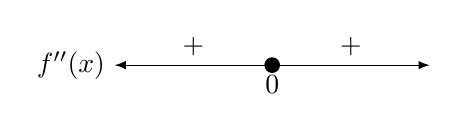
\begin{tikzpicture}[yscale=0.1]
          \draw[<->] (-2,0) -- (2, 0);
          \node[left] at (-2,0) {$f''(x)$};
          \foreach \x in {0}
            \draw[shift={(\x,0)},color=black] (0pt,3pt) -- (0pt,-3pt) node[below] {$\x$};
          \foreach \x in {0}
            \node[circle, fill=black, inner sep=2pt] at (\x,0) {};
          \node[above] at (-1, 0) {$+$};
          \node[above] at (1, 0) {$+$};
        \end{tikzpicture}
      \end{center}
      From the sign chart, we can conclude that:
      \begin{itemize}
        \item $f$ is concave up on $(-\infty, 0)$ and $(0, \infty)$, since $f''$ is positive on those intervals
          \footnote{We could say that $f$ is concave up on $(-\infty, \infty)$.}
        \item $f$ is never concave down, because $f''$ is never negative
        \item $f$ has no inflection points, because $f$ never changes concavity
      \end{itemize}
    \end{solution}

  \item
    \begin{problem}[\vfill\newpage]
      Sketch a possible graph of $f$.
    \end{problem}

    \begin{solution}
      First, let's sketch a graph that's consistent with the information we found in part (a). We know
      $f$ should be decreasing on $(-\infty, 2)$ and increasing on $(2, \infty)$. 
      There should be a horizontal tangent at the turning point, but we'll smooth it out later.

      \begin{center}
        \begin{tikzpicture}
          \begin{axis}[ytick=\empty, xtick={2}]
            \addplot+[domain=-4:2, dashed] {-x+1};
            \addplot+[domain=2:6, dashed] {x-3};
          \end{axis}
        \end{tikzpicture}
      \end{center}

     Note that we don't know where the $x$-intercept(s) or $y$-intercept actually are.

     Now let's revise our graph to represent the information we found in part (c). We know that $f$ should
     be concave up on $(-\infty, 0)$ and $(0, \infty)$. 
     \begin{center}
        \begin{tikzpicture}
          \begin{axis}[ytick=\empty, xtick={2}, tick label style={fill=white}, axis on top]
            \addplot+[domain=-4:5] {x^4/4 -8*x + 5};
          \end{axis}
        \end{tikzpicture}
      \end{center}
      
    \end{solution}

    

  \end{enumerate}

\end{enumerate}
\end{document}
